\documentclass[12pt]{article}
\usepackage{float}
\usepackage{amsthm}
\usepackage{amsmath}
\usepackage{lineno}
\usepackage{cite}
\usepackage{amssymb,graphics,color,cite,amsmath}
\usepackage{subfig}
\usepackage{graphicx}
\usepackage{epsfig}
\usepackage{psfrag}
\usepackage[margin=0.75in]{geometry}
\usepackage{float}
\usepackage{afterpage}

\usepackage[noblocks]{authblk}
%\usepackage{natbib}
\usepackage{stackengine}

\usepackage{xspace}
\newcommand{\themename}{\textbf{\textsc{metropolis}}\xspace}

\renewcommand{\(}{\left (}
\renewcommand{\)}{\right )}
\renewcommand{\vec}[1]{\boldsymbol{#1}}

\begin{document}

\title{Proposal: Synchronization of Two Cellular Circadian Rhythms}
\date{}
\author[1]{Zeshun Zong}
\author[2]{Yuliang Shi}
\affil[1,2]{\footnotesize Courant Institute of Mathematical Sciences, New York University, New York, New York, United States of America}

\maketitle


\section{Introduction}

\hspace{5mm} In human cells, DNA in nucleus is first transcripted to mRNA, and then translated to various proteins that play essential rules in our body. This process is happening massively and consecutively in every cell. Here we consider a particular type of pathway: the expression of a clock gene. This type of pathway has a negative feedback. Some proteins expressed by the genes will re-enter the nucleus and inhibit the transcription process and therefore slow down the rate of protein expression.

\section{Mathematical Model}

\subsection{Basic Setups}

\hspace{5mm} To show the basic setups of our proposed model, we first introduce some notions:
\begin{itemize}
  \item $m_n$: number of mRNAs inside the nucleus;
  \item $m_c$: number of mRNAs in the cytoplasm;
  \item $p_n$: number of protein molecules inside the nucleus;
  \item $p_c$: number of protein molecules in the cytoplasm;
  \item $\alpha$: transcription rate when no proteins are binding;
  \item $r$: total number of sites on which the protein can bind;
  \item $K$: the equilibrium constant of the reaction of protein binding to DNA molecules;
  \item $\gamma_m$: the rate at which mRNAs inside the nucleus are transported to cytoplasm;
  \item $\delta_m$: the degradation rate of mRNAs in cytoplasm;
  \item $\gamma_p$: the rate at which the protein molecules in the cytoplasm are transported into nucleus;
  \item $\delta_p$: the degradation rate of this protein inside nucleus;
\end{itemize}

In our model, we assume that the protein can inhibit the transcription by binding to the DNA molecules on several pre-determined sites. The transcription continues if and only if none of the sites are occupied. \\

The pathway of this protein expression is shown in Figure 1, and reaction rates are marked on the arrows which indicate corresponding reactions. DNA is first transcripted to mRNA, and we denote the quantity of mRNA in nucleus by $m_n$. Then, at a rate of $\gamma_m m_n,$ mRNAs are transported to cytoplasm. mRNAs degrade in cytoplasm at a rate of $\delta_m m_c,$ while the translation process takes a rate of $\beta m_c$. The amount of protein in cytoplasm is $p_c$. The protein molecules in cytoplasm are transported into nucleus at a rate of $\gamma_p p_c$. Some proteins degrade in the nucleus at a rate of $\delta_p p_n$, while the others might bind to DNA's and inhibit the transcription. Finally we see that the rate of transcription is $\alpha \{\frac{K}{K + P_n / V_n}\}^r.$ We can think of $\frac{K}{K + P_n / V_n}$ as the possibility that one particular site is not occupied, so it being raised to $r^\text{th}$ power is the probability that all sites are not occupied.


\begin {figure}[t]
	\centering
	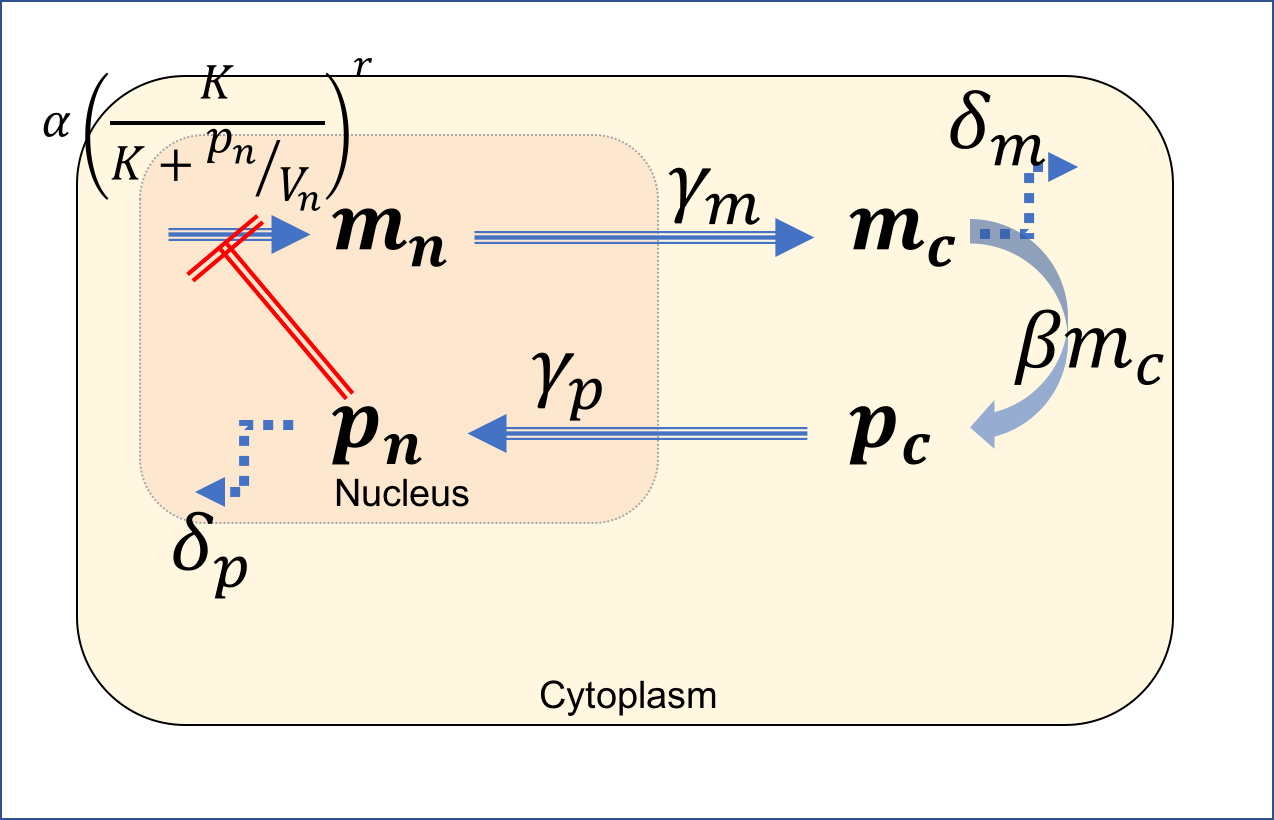
\includegraphics[width=0.5\textwidth]{pathway.png}
	\caption*{\small Figure 1: a schematic cellular clock}
\end {figure}

\subsection{Modeling Topics}

\begin{itemize}
    \item First, we would like to demonstrate the circadian rhythm of a cell with the simplified procedure illustrated above. By choosing parameters carefully, we may be able to show some periodical oscillations.
    \item Another interesting topic is to illustrate how different (adjacent) cells could influence each other in term of their circadian rhythms. In human body, information can be exchanged among cells. In particular, we would like to explore how the flow of information can influence the circadian rhythms among two or more cells. To simplify things in our model, we will get started by considering two cells, and the flows of protein between two cells are going to be modeled as through diffusion. Although in real life the mechanism of exchanging information is much more complicated, we believe that our simplified diffusion model should convey the similar idea. See Figure 2.
    \item Also, if the two cells have different periods, can they synchronize themselves to a shared period when we introduce the protein diffusion? In real life, since cells are different, it is very common to have different circadian rhythms for different cells. It is the exchange of information that allows cells to together maintain our biological clock, whose period is approximately 24 hours. We propose to delineate this phenomenon in our simple model. We expect to see that, for example, if one cell has a circadian period of 24h, while the other 22h, the diffusion of proteins would gradually drag them together and eventually both cells would run on some synchronized period of, say, 23h. If they do converge to a shared rhythm, what the period of the shared rhythm would also be an interesting topic. Moreover, we are expecting convergence only when the rhythmic period of the two cells are not drastically different. What would happen if one has a period which is a multiple of the other? These questions shall be explored in our model.
    \item Finally, as what will be discussed in the paragraph below, there are both a deterministic version and a stochastic version to do the simulation. It would also be interesting to compare the difference of those two modeling methods. We are suspecting that in the stochastic version, it would be easier (or it takes shorter time) for the two cells to be synchronized, since noise in this case can help to stabilize the system. Such questions shall be visited if time permits.
\end{itemize}

\begin {figure}[t]
	\centering
	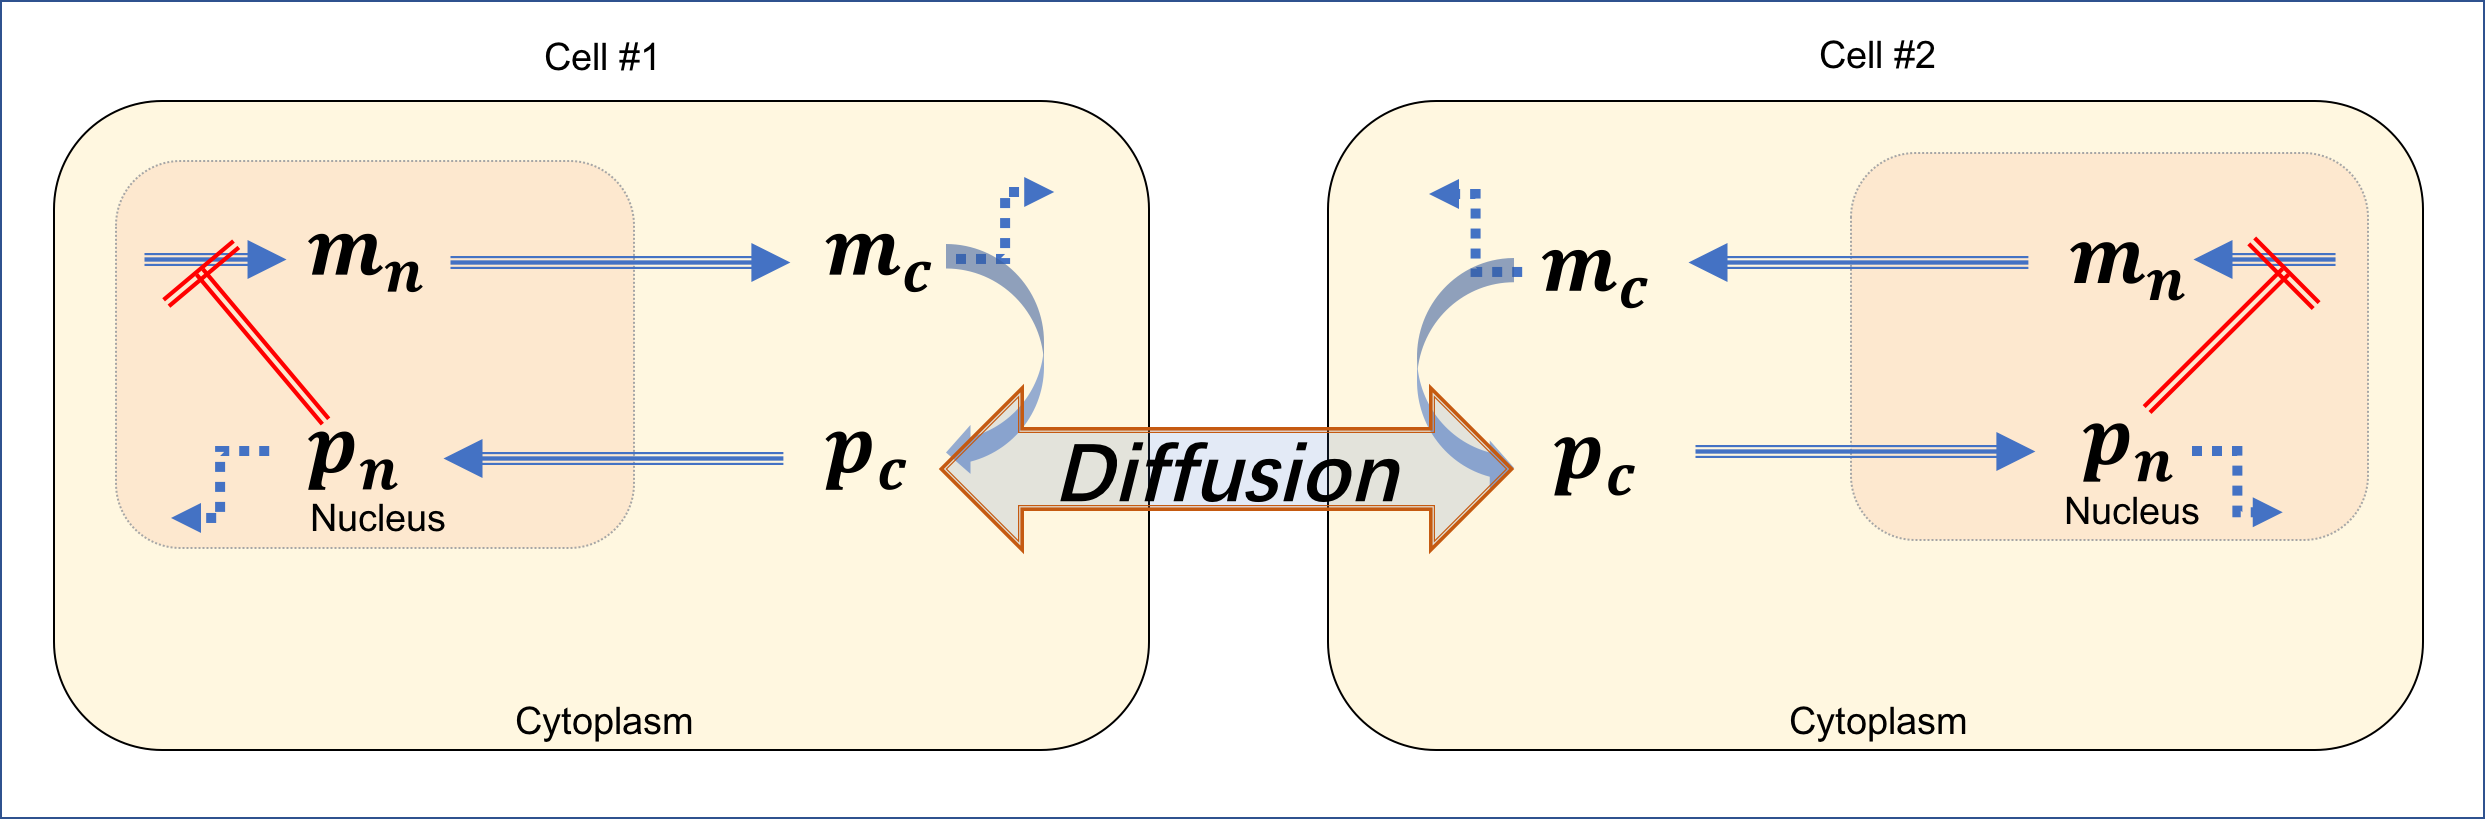
\includegraphics[width=0.6\textwidth]{two_cells.png}
	\caption*{\small Figure 2}\label{Fig:nref=1}
\end {figure}

\subsection{Modeling Methodology}

\subsubsection{Deterministic Version}
There are two ways to simulate such a circadian rhythm. One way is to view a set of molecules as continuous entity (while the number of them could only be integers), and then describing the system using differential equations. However, viewing the set of molecules as a continues entity would very possibly be a good modeling technique, as the number of molecules are quite large. Hence, by solving systems of ODE's numerically, we could observe how the rhythm varies.

\subsubsection{Stochastic Version}
The other way is a stochastic version, in which we are proposing a way to \textit{``perform''} a system of reactions by randomly choosing a action for each time step with respect to some predetermined probability distributions. We hope this could demonstrate how will the amount of molecules changes at each time step. Moreover, we are also planning to add some random noises to the system of reactions.

\subsubsection{Modeling Diffusion}
We are proposing that the rate of diffusion is proportional to the difference of the concentrations of proteins among two different cells. To be more specific, if $p_c$ has a higher concentration in cell 1 than in cell 2, then we expect a net flow of $p_c$ molecules from cell 1 to cell 2. The exact rule for diffusion shall be given by
\begin{equation}
	\frac{d {p_c^1}}{dt} = -\lambda ({p_c^1 - p_c^2})
\end{equation}
and \begin{equation}
	\frac{d {p_c^2}}{dt} = -\frac{d {p_c^1}}{dt},
\end{equation}
where $p_c^1$ and $p_c^2$ are the number of protein molecules in cell 1 and cell 2 respectively, and $\lambda$ is some constant. Several questions remain interesting.

Suppose the two cells are exactly the same, i.e. they are governed by parameters with the same values, then they should have the same rhythmic period. However, they might not be initialized at the same time. So there will be a phase difference between the two rhythms of the cells. If the two cells are isolated, it is clear that both of them would follow its own period, so although they have the same period, the phase difference would be kept. Now if we allow communication between the two cells through protein diffusion, we are expecting to observe that the phase difference would go to zero and eventually the two cells will obey a synchronized circadian rhythm. We propose to simulate such a process in our project.

\section{Numerical Methodology}
To model this, we are planning to use Forward Euler Method and Newton's Method, and some others (e.g. Backward Euler Method) when it requires:
\begin{itemize}
    \item Euler's Method:\\
    For example, Euler's Method will be used to modeling and approximating $m_n$, $m_c$, $p_n$, $p_c$ with respect to a system of ODE's.
    \item Newton's Method:\\
    We are proposing Newton's Method for some circumstances where we need to find the optimal rate such that it gives us desired synchronized period or fast convergence rate.
\end{itemize}




\begin{thebibliography}{9}

	\bibitem{Wang}
	Wang, Guanyu and Peskin, Charles S (2018).
	The minimum energy of bending as a possible explanation of the biconcave shape of the human red blood cell.
	\textit{Physical Review E,}
	97(6).


\end{thebibliography}

\end{document}
